\section{Databases for the Generic T-tail Transport Aircraft} \label{sec:gtt_dbs}

Thus far, the examples of probabilistic databases has been focused on the baseline aerodynamics of the aircrafts in question. 
This section will focus on controls databases which define the aircraft's response to a control surface deflection by providing the resulting rotational moments that are imparted. 
As mentioned in Section \ref{subsec:gtt_cfd_data_gen}, the difficulty in modeling control surface deflections precludes the use of CFD simulation data in building these controls databases. 
Consequently, these databases can be, at most, two-fidelity ones with AVL simulations and wind tunnel experiments as the data sources. 
A number of visualizations of the GP regressions are presented in this section.
To showcase certain advantages of using multi-fidelity data, single-fidelity GP results using AVL data and WT data in isolation are presented.
This is contrasted with the two-fidelity GP results that use both sets of data. 

In the interest of brevity and since the maneuver of interest focuses on the roll-authority of the aircraft, these visualizations will present the roll moment imparted due to aileron deflection ($C_{l{\delta_a}}$).
This is just one of the 18 coefficients (Table \ref{tab:control_db}) that define the aircraft's control behavior, but is the most pivotal for the maneuver of interest. 

\subsection{Single-fidelity Databases}
The results of the single-fidelity GP regression performed on AVL data and wind tunnel data are presented in Figures \ref{fig:gtt_avl_ctrl_gps} and \ref{fig:gtt_wt_ctrl_gps} respectively. 
With controls databases, a new input variable defining the control surface deflection angle ($\delta_*$) is used in addition to $\alpha$ and $\beta$ .
This makes visualizing the results of 3-dimensional GP in 3D space challenging. 
For both sets of figures, 4 surfaces or lines are shown in the first three subfigures. 
Each individual line or surface corresponds to the GP prediction at a particular aileron deflection angle.
For each of the figures, they are stacked in order of increasing deflection angle, where the angles are $\delta_a \in \{-25^\circ, -10^\circ, 10^\circ, 25^\circ\}$. 
These deflection angles are chosen because the wind tunnel experiments were carried out with these aileron deflection angles. 

\begin{figure}
    \centering
    \begin{subfigure}[\label{subfig:gtt_avl_ctrl_surf}3-Dimensional function in $\alpha$, $\beta$, and $\delta_a$] {
        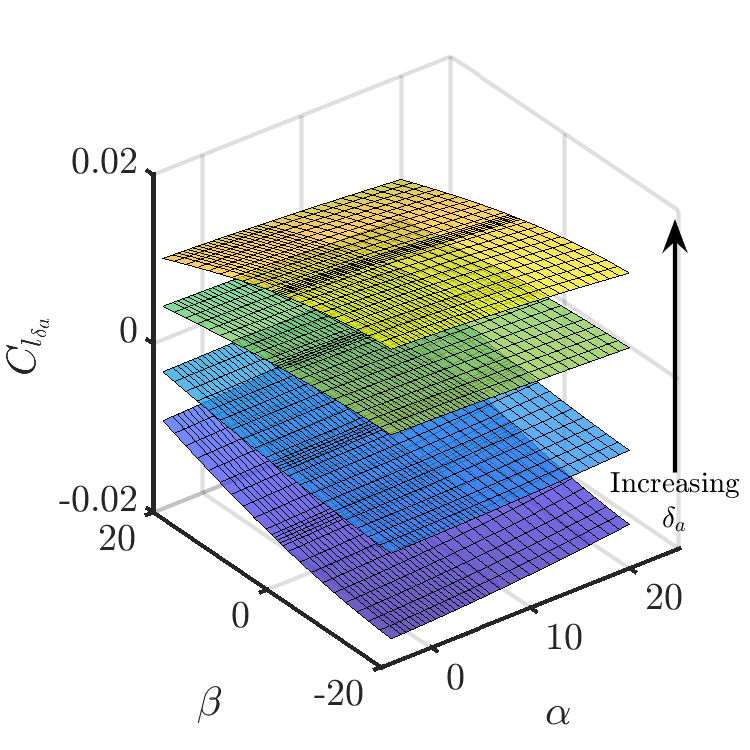
\includegraphics[trim=0 0 0 0, clip, width=.48\textwidth]{code/image_gen/gmatt/1f/avl/images/gps/CRMAIL.png} }
    \end{subfigure}
    \hfill
    \begin{subfigure}[\label{subfig:gtt_avl_ctrl_beta}Variation in $\beta$ at $\alpha=8^\circ$]{
        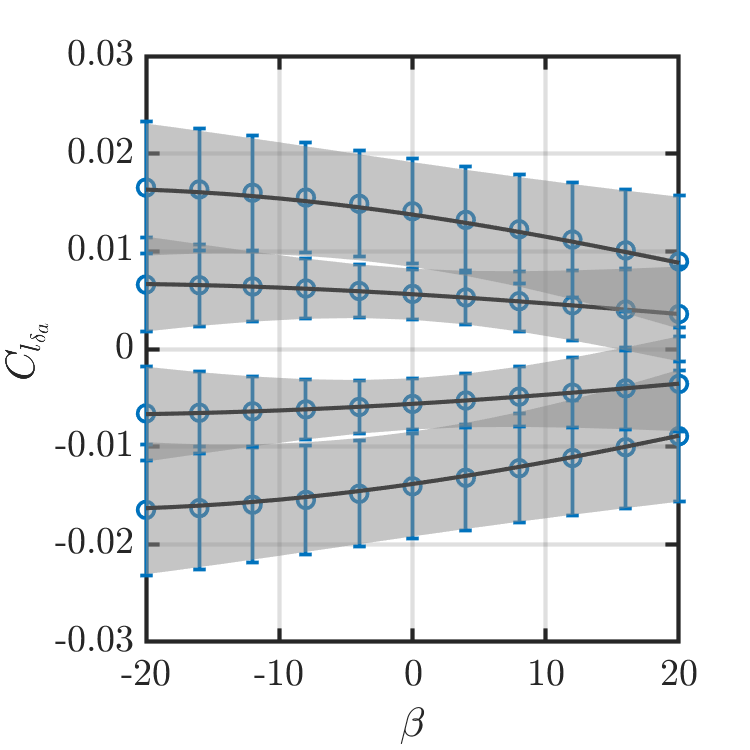
\includegraphics[trim=0 0 0 0, clip, width=.48\textwidth]{code/image_gen/gmatt/1f/avl/images/gps/CRMAIL_alpha=8.png}
    }
    \end{subfigure}
    \hfill
    \begin{subfigure}[\label{subfig:gtt_avl_ctrl_alpha}Variation in $\alpha$ at $\beta=4^\circ$]{
        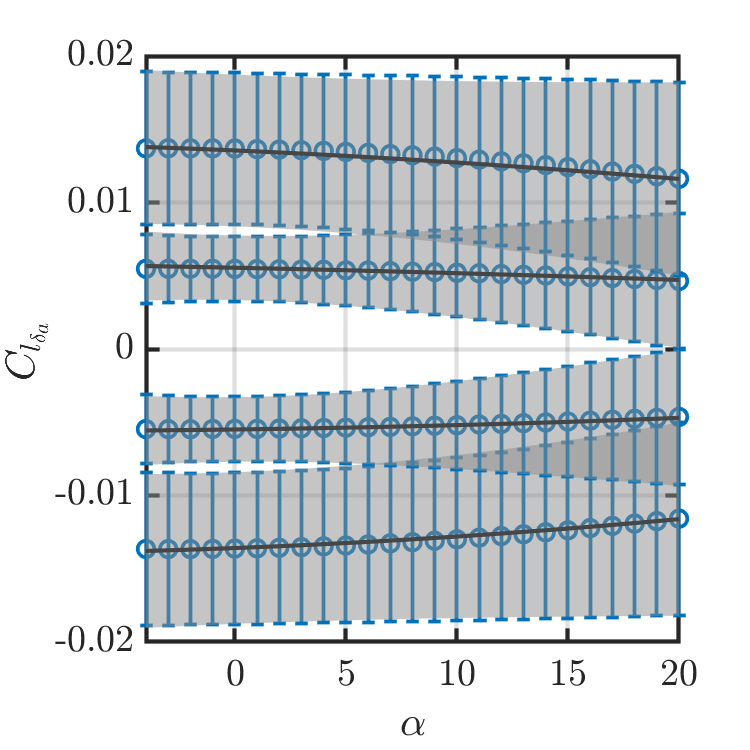
\includegraphics[trim=0 0 0 0, clip, width=.48\textwidth]{code/image_gen/gmatt/1f/avl/images/gps/CRMAIL_beta=4.png} 
    }
    \end{subfigure}
    \hfill
    \begin{subfigure}[\label{subfig:gtt_avl_ctrl_defl}Variation in $\delta_a$ at $\alpha = 8^\circ$ and $\beta=4^\circ$]{
        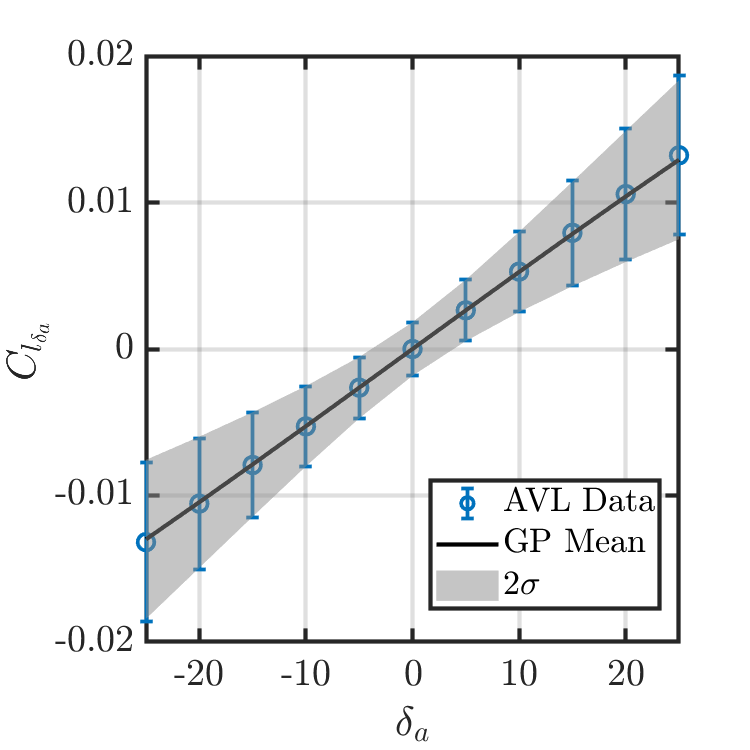
\includegraphics[trim=0 0 0 0, clip, width=.48\textwidth]{code/image_gen/gmatt/1f/avl/images/gps/CRMAIL_alpha=8_beta=4.png} 
    }
    \end{subfigure}
    \caption{Visualization of the 3-Dimensional AVL data and resulting single-fidelity GP for the rolling moment due to aileron deflections. \label{fig:gtt_avl_ctrl_gps}}
\end{figure}

\begin{figure}
    \centering
    \begin{subfigure}[\label{subfig:gtt_wt_ctrl_surf}3-Dimensional function in $\alpha$, $\beta$, and $\delta_a$] {
        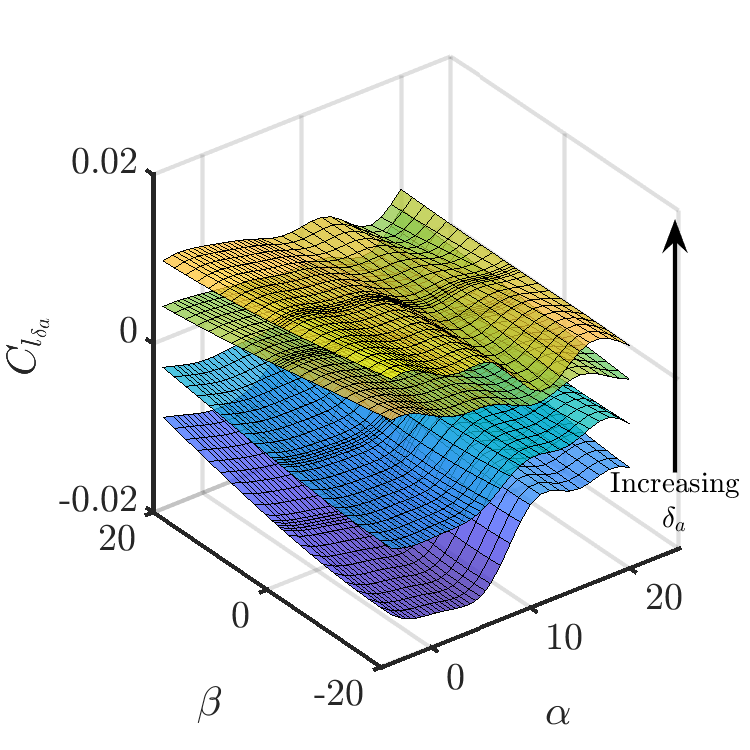
\includegraphics[trim=0 0 0 0, clip, width=.48\textwidth]{code/image_gen/gmatt/1f/wt/images/gps/CRMAIL.png} }
    \end{subfigure}
    \hfill
    \begin{subfigure}[\label{subfig:gtt_wt_ctrl_beta}Variation in $\beta$ at $\alpha=8^\circ$]{
        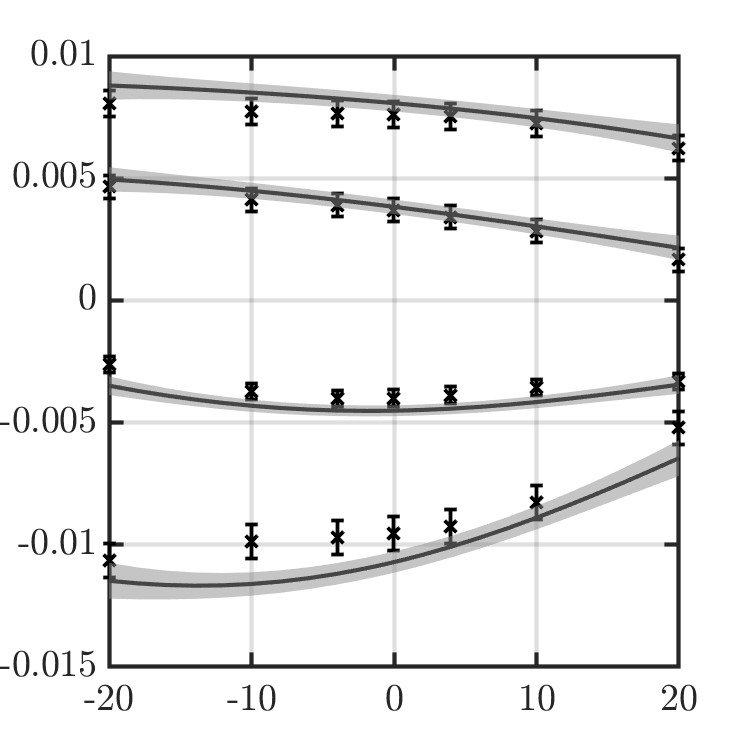
\includegraphics[trim=0 0 0 0, clip, width=.48\textwidth]{code/image_gen/gmatt/1f/wt/images/gps/CRMAIL_alpha=8.png}
    }
    \end{subfigure}
    \hfill
    \begin{subfigure}[\label{subfig:gtt_wt_ctrl_alpha}Variation in $\alpha$ at $\beta=4^\circ$]{
        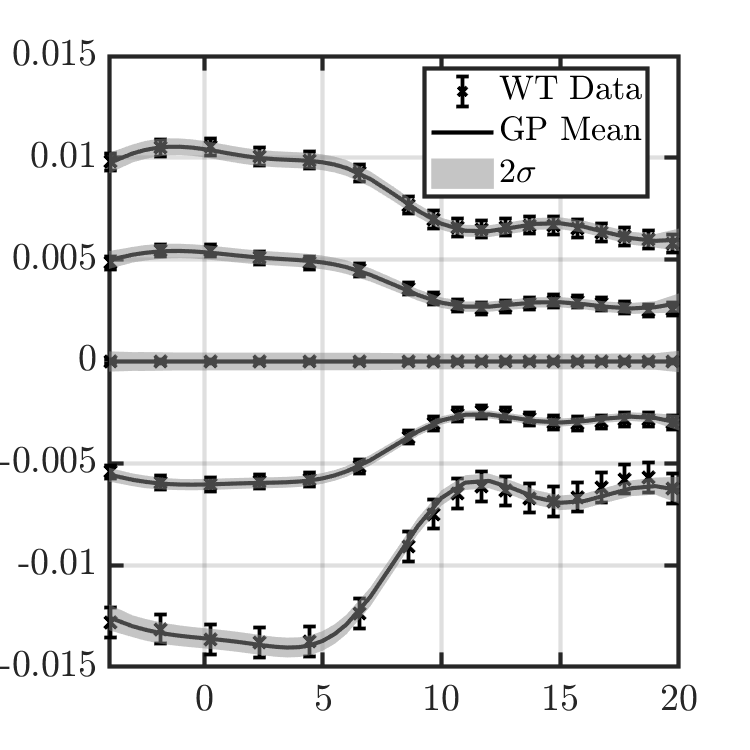
\includegraphics[trim=0 0 0 0, clip, width=.48\textwidth]{code/image_gen/gmatt/1f/wt/images/gps/CRMAIL_beta=4.png} 
    }
    \end{subfigure}
    \hfill
    \begin{subfigure}[\label{subfig:gtt_wt_ctrl_defl}Variation in $\delta_a$ at $\alpha = 8^\circ$ and $\beta=4^\circ$]{
        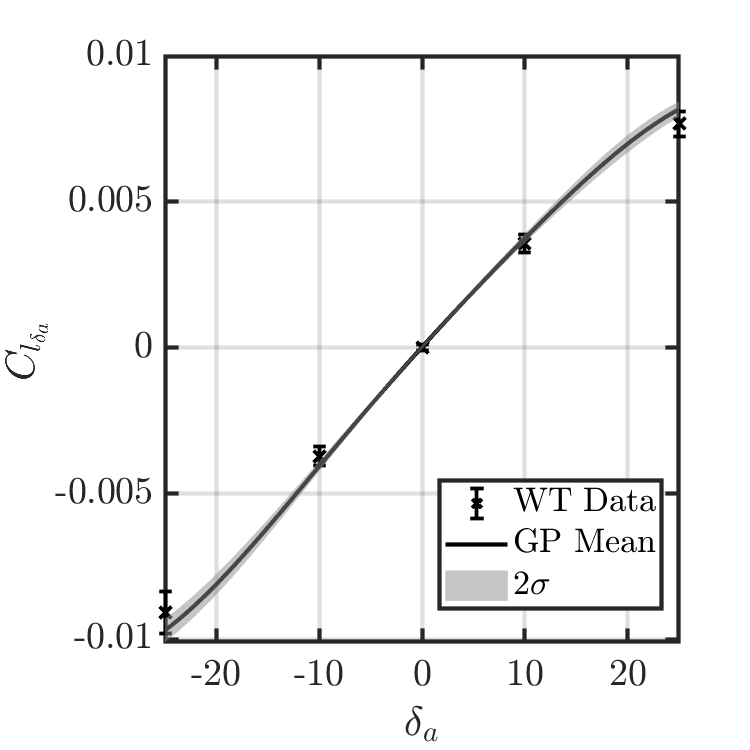
\includegraphics[trim=0 0 0 0, clip, width=.48\textwidth]{code/image_gen/gmatt/1f/wt/images/gps/CRMAIL_alpha=8_beta=4.png} 
    }
    \end{subfigure}
    \caption{Visualization of the 3-Dimensional WT data and resulting single-fidelity GP for the rolling moment due to aileron deflections. \label{fig:gtt_wt_ctrl_gps}}
\end{figure}

Figures \ref{subfig:gtt_avl_ctrl_surf} and \ref{subfig:gtt_wt_ctrl_surf} present stacks of surfaces where each surface represents $C_{l{\delta_a}}$ as a function of $\alpha$ and $\beta$ at a particular aileron deflection angle ($\delta_a$).
Explicitly, the lowest surface in both figures corresponds to $\delta_a = -25^\circ$.
At the lowest level, the AVL data does capture the general trend of increasing $\delta_a$ leading to increased rolling moment but there is a clear contrast in the linear trends that are learned from the AVL data and the non-linear trends represented in the wind tunnel data. 

In Figures \ref{subfig:gtt_avl_ctrl_beta} and \ref{subfig:gtt_wt_ctrl_beta}, the angle of attack is kept constant, $\alpha = 8^\circ$ and $C_{l{\delta_a}}$ is represented as a function of $\beta$ at different values of $\delta_a$. 
For the AVL-based results (Figure \ref{subfig:gtt_avl_ctrl_beta}), the uncertainty in the data is represented by the blue circles and the associated error bars.
These are quite large and they result in overlap in the gray $2\sigma$ uncertainty estimates at different $\delta_a$. 
For the WT-based results (Figure \ref{subfig:gtt_wt_ctrl_beta}) the uncertainty is a lot lower but there is some discrepancy in the data points (black crosses) and the GP mean estimate (solid black line).
This is not an error in the GP, rather a consequence of the multi-dimensional hyper-parameters that are learned while maximizing the log-liklihood of the model (Equation \ref{equ:hyp_param_sf}. 
Regularization prevents over-fitting to the data. 

For Figures \ref{subfig:gtt_avl_ctrl_alpha} and \ref{subfig:gtt_wt_ctrl_alpha}, the angle of slideslip is kept constant, $\beta=4^\circ$ and $C_{l{\delta_a}}$ is represented as a function of $\alpha$ at different values of $\delta_a$.
There is a similar overlap of the uncertainty estimate for the AVL-based GP, and a capturing of non-linear trends by the WT-based GP. 

Figures \ref{subfig:gtt_avl_ctrl_defl} and \ref{subfig:gtt_wt_ctrl_defl} present $C_{l{\delta_a}}$ as a function of $\delta_a$ when $\alpha = 8^\circ$ and $\beta = 4^\circ$.
There is a distinctly linear relationship between the rolling moment and the aileron deflection. 
While the AVL based GP respects the uncertainty in the data across the domain, the WT-based GP predicts increased uncertainty between data points. 
In these areas the uncertainty in the model parameters is surpassing the uncertainty in the data.
This indicates a need for additional data between the current set of aileron deflection angles for which wind tunnel data is available.
This is something that is addressed by using the multi-fidelity framework.

\subsection{Multi-fidelity Databases}
The limited wind tunnel data points can be augmented by the lower-fidelity AVL data to create a better surrogate model.
Figure \ref{fig:gtt_2f_ctrl_gps} continues in the vein of the previous figures with stacks of lines and surfaces representing the rolling moment at different aileron deflection angles. 
When compared to the single-fidelity WT-based GP shown in Figure \ref{fig:gtt_wt_ctrl_gps}, the results are similar with the notable exception of Figure \ref{subfig:gtt_2f_ctrl_defl}.
When the abundant AVL data is used to supplement the sparse WT data in the aileron deflection dimension, the ballooning of the uncertainty estimates between data points disappears. 
The uncertainty estimates across the domain is reduced without using any more high-fidelity data. 

\begin{figure}
    \centering
    \begin{subfigure}[\label{subfig:gtt_2f_ctrl_surf}3-Dimensional function in $\alpha$, $\beta$, and $\delta_a$] {
        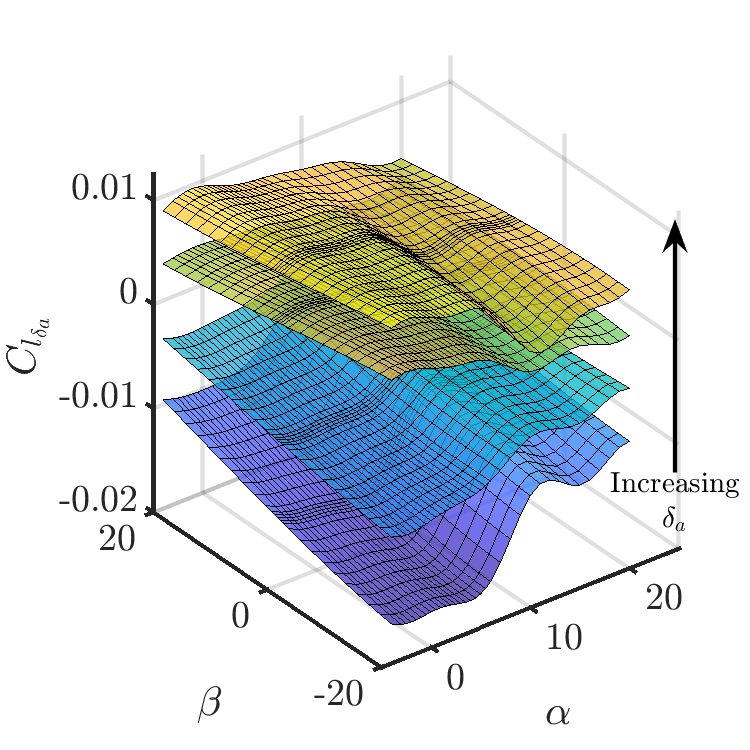
\includegraphics[trim=0 0 0 0, clip, width=.48\textwidth]{code/image_gen/gmatt/3f/images/gps/CRMAIL.png} }
    \end{subfigure}
    \hfill
    \begin{subfigure}[\label{subfig:gtt_2f_ctrl_beta}Variation in $\beta$ at $\alpha=8^\circ$]{
        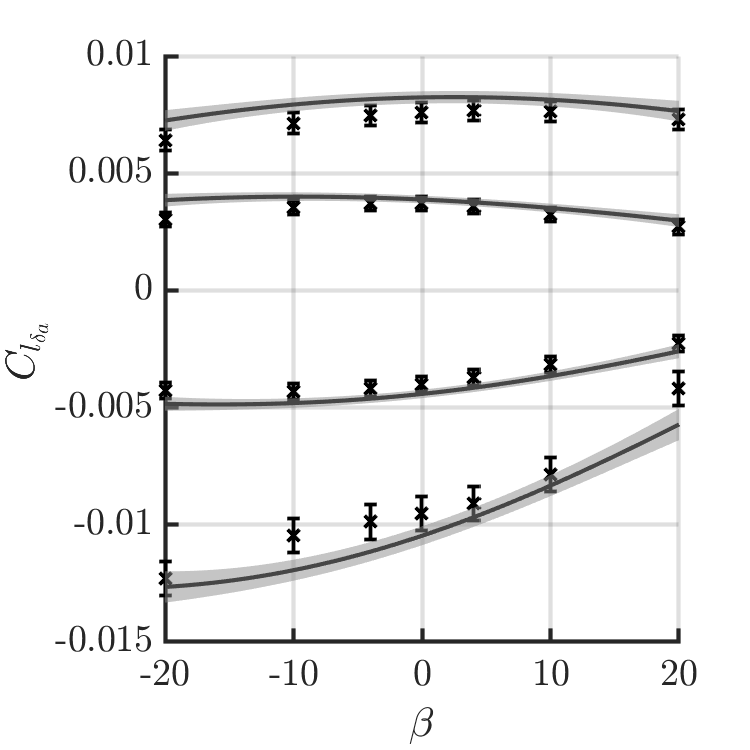
\includegraphics[trim=0 0 0 0, clip, width=.48\textwidth]{code/image_gen/gmatt/3f/images/gps/CRMAIL_alpha=8.png}
    }
    \end{subfigure}
    \hfill
    \begin{subfigure}[\label{subfig:gtt_2f_ctrl_alpha}Variation in $\alpha$ at $\beta=4^\circ$]{
        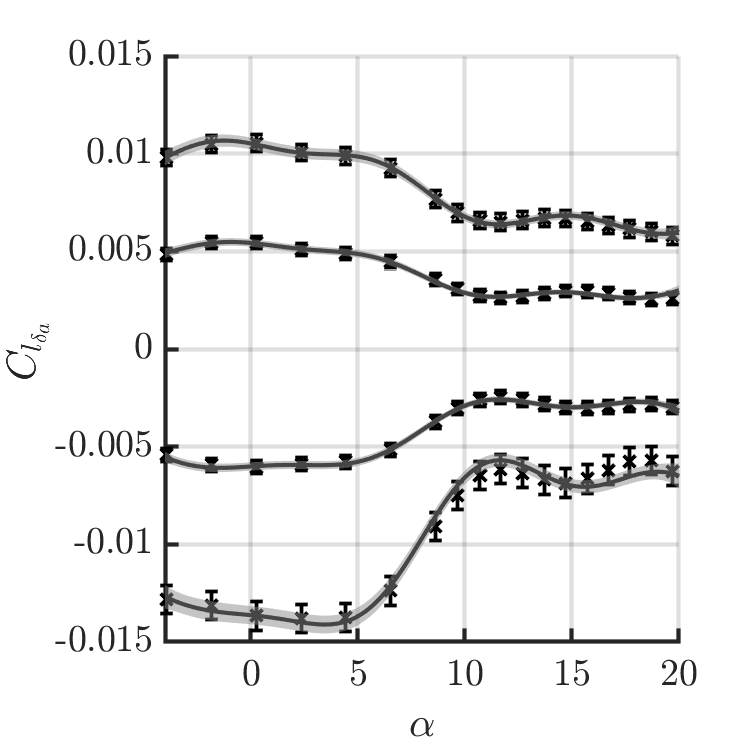
\includegraphics[trim=0 0 0 0, clip, width=.48\textwidth]{code/image_gen/gmatt/3f/images/gps/CRMAIL_beta=4.png} 
    }
    \end{subfigure}
    \hfill
    \begin{subfigure}[\label{subfig:gtt_2f_ctrl_defl}Variation in $\delta_a$ at $\alpha = 8^\circ$ and $\beta=4^\circ$]{
        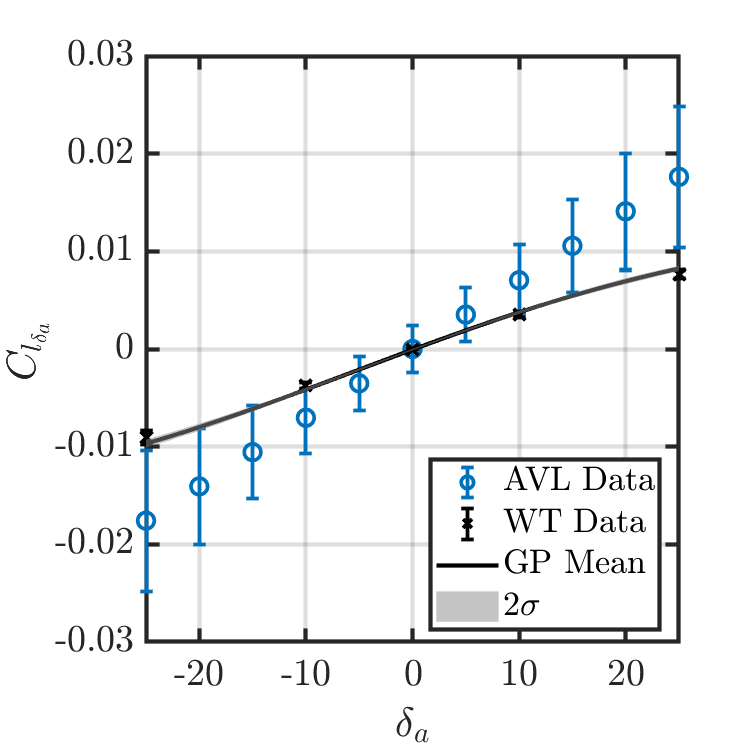
\includegraphics[trim=0 0 0 0, clip, width=.48\textwidth]{code/image_gen/gmatt/3f/images/gps/CRMAIL_alpha=8_beta=4.png} 
    }
    \end{subfigure}
    \caption{Visualization of the 3-Dimensional AVL and WT data, and the resulting two-fidelity GP for the rolling moment due to aileron deflections. \label{fig:gtt_2f_ctrl_gps}}
\end{figure}

This is a significant advantage of using multi-fidelity data, but there is a caveat.
The lower fidelity data needs to capture some relevant trend in the high-fidelity data. 
If the lower-fidelity trends contradict those seen in the high-fidelity data, then the low-fidelity data only serves to corrupt the GP predictions. 
The multi-fidelity GP is trained on the difference between the low-fidelity data and the high-fidelity data. 
If there is no correlation between the low-fidelity and the high-fidelity data, then the difference between the two sets of data provides no useful information and only serves to add noise to the system. 
This, in turn, would prevent the multi-fidelity fit from performing as well, or better than, the single-fidelity fits. 